\documentclass[subsection=false, compress]{beamer}
\setbeamertemplate{footline}[frame number] % numerar slides
\setbeamertemplate{navigation symbols}{} % retirar barra de navega��o
\setbeamertemplate{background}{\tikz[overlay,remember picture]\node[opacity=1]at (current page.center){
\includegraphics[width=\paperwidth, height=\paperheight]{Figures/water-mark}};}

\mode<presentation>
% \usetheme{Singapore}
%\usefonttheme{structurebold}
%\usebeamercolor[fg]{section in sidebar}

\ifdefined\hyperref  

\usepackage[brazil]{babel}
\usepackage[latin1]{inputenc}
\usepackage{subfig}
\usepackage{graphicx}
%\usepackage{subcaption}  
\usepackage{pgfpages}
\usepackage{ifpdf}   
\usepackage{multimedia}  
\usepackage{color}   
\usepackage{url} 
\usepackage{hyperref}
\usepackage{lastpage}
\usepackage{listings}
\usepackage{listing}
\usepackage{nameref}
\usepackage{array}
\usepackage{marvosym} 
\usepackage{multicol} 
\usepackage{pifont}
\usepackage{marvosym}
\usepackage{cancel}
%\usepackage{enumitem} 
%\usepackage{minted}
%\usepackage{subfigure}
%\usepackage{xmpmulti}
%\usepackage{animate}
\usepackage[export]{adjustbox}
\usepackage{changepage}
\usepackage{lipsum}
\usepackage{tikz}
\usepackage{kantlipsum}

\definecolor{erick}{HTML}{7CFC00}
\definecolor{suzane}{HTML}{006400}


\lstset{%
	linewidth=\textwidth,%framed box is the text size 
	xleftmargin=.10in,
	xrightmargin=.10in, 
	frame=trbl, 
	columns=flexible, 
	captionpos=t, 
	upquote=false,
	basicstyle=\footnotesize\ttfamily,
	firstnumber=1,% 
	numberfirstline=false,% 
	numbers=left,%
	numberstyle=\tiny,% 
	stepnumber=1,%
	numbersep=5pt,% 
	backgroundcolor=\color{blue!15},% 
	tabsize=4,% 
	keywordstyle=\color{green!65!black},% 
	commentstyle=\color{blue},% 
	stringstyle=\color{magenta},% 
	breaklines=true,% 
	emph={label},%
	abovecaptionskip=10pt,% 
	belowcaptionskip={\abovecaptionskip},%
	showstringspaces=false, 
	escapeinside=@@,%
	literate={�}{{\^{E}}}1
}%
\usepackage{textpos} % package for the positioning

% position the logo
% \addtobeamertemplate{frametitle}{}{%
% 	\begin{textblock*}{100mm}(\textwidth,6.70cm)
		% 
\includegraphics[height=1.00cm,width=1.00cm,keepaspectratio]{Figures/logo_ufpa}
	% \end{textblock*}
	%\begin{textblock*}{100mm}(-0.80cm,-0.25cm)
	%\begin{textblock*}{100mm}(-0.80cm,6.90cm)
	%	
\includegraphics[height=1.00cm,width=1.00cm,keepaspectratio]{Figures/ihc}
	%\end{textblock*}
% }

%%\pgfdeclareimage[width=0.85cm, height=1.10cm]{ufpa}{Figures/logo_ufpa}
%\pgfdeclareimage[width=1.60cm, height=1.00cm]{ufpa}{Figures/foot_img}
%\logo{\pgfuseimage{ufpa}}

\hypersetup{
    pdftitle={Uma Proposta de Controle Alternativo do Mouse Centrado na Cabe�a do Usu�rio}
	pdfauthor={Jo�o Victor da Silva Dias Canavarro}
}
\fi

\makeatletter
\newcommand*{\currentname}{\@currentlabelname}
\makeatother

% http://tex.stackexchange.com/questions/50286/beamer-singapore-theme-follow-up-line-above-footline-and-hide-footline-for-si
%\setbeamercolor{footlinerule}{use=structure,bg=structure.fg!25!bg,green}
\setbeamertemplate{footline}
{%
	\begin{beamercolorbox}[wd=\paperwidth,ht=0.5ex,dp=0ex,center]{footlinerule}
	\end{beamercolorbox}%
	\begin{beamercolorbox}[wd=\paperwidth,ht=0.6ex,dp=0ex,center]{empty}
	\end{beamercolorbox}%
	\leavevmode%
	\hbox{%

	\begin{beamercolorbox}[wd=.20\paperwidth,ht=2.25ex,dp=2ex,center]{author in head/foot}%
		\usebeamerfont{author in head/foot}%
		\insertshortauthor\hspace{1em}%(FCT/\insertshortinstitute)
	\end{beamercolorbox}%

	\begin{beamercolorbox}[wd=.45\paperwidth,ht=2.25ex,dp=2ex,right]{title in head/foot}%
		\usebeamerfont{title in head/foot}
		\insertshorttitle
	\end{beamercolorbox}%

	\begin{beamercolorbox}[wd=.20\paperwidth,ht=2.25ex,dp=2ex,right]{author in head/foot}%
		\usebeamerfont{author in head/foot}%
		\textbf{\textcolor{black}{\currentname}}
	\end{beamercolorbox}%

	\begin{beamercolorbox}[wd=.10\paperwidth,ht=2.25ex,dp=2ex,right]{date in head/foot}%
		\textbf{\textcolor{black}{\insertframenumber{} de \inserttotalframenumber\hspace*{1ex}}}
	\end{beamercolorbox}}%
	\vskip0pt%
}%

%\title[Universal Remote Control System with AGR]
%{\Large A Proposal of a Universal Remote Control System Based on Head Movements}
%
%\author[Cassio T. Batista]
%{\large
%\textbf{Cassio Trindade Batista}\\
%Erick Modesto Campos\\
%Nelson Cruz Sampaio Neto
%\vspace{.2cm}
%}

%\institute[UFPA]{
%\small
%Universidade Federal do Par�\\[1pt]
%%Programa de P�s-Gradua��o em Ci�ncia da Computa��o\\[1pt]
%Laborat�rio de Visualiza��o, Intera��o e Sistemas Inteligentes\\[1pt]
%Bel�m -- Par� -- Brazil\\[1pt]
%\begin{figure}
%	
\includegraphics[width=.13\textwidth]{Figures/logo_ufpa}
%\end{figure}
%\vspace{-0.40cm}
%}
%\date{
%\small
%25 de outubro de 2017
%}
% \title[Acionador Externo de Baixo Custo Baseado em Sopro]
\title[Controle Alternativo do Mouse Centrado na Cabe�a do Usu�rio]
% {\Large Uma Proposta de Acionador Externo de Baixo Custo Baseado em Sopro}
{\Large Uma Proposta de Controle Alternativo do Mouse Centrado na Cabe�a do Usu�rio}
\author[ Jo�o V. Canavarro ]
{\large \textbf{Jo�o Victor da Silva Dias Canavarro}\vspace{.2cm}}

\institute[UFPa]{
\small
Instituto de Ci�ncias Exatas e Naturais\\[1pt]
Faculdade de Computa��o\\[1pt]
Laborat�rio de Visualiza��o, Intera��o e Sistemas Inteligentes\\[1pt]
% Aluno: Jo�o Victor da Silva Dias Canavarro
Orientador: Prof. Dr. Nelson Cruz Sampaio Neto \\
% \begin{figure}
% 
\includegraphics[width=.13\textwidth]{Figures/logo_ufpa}
% \end{figure}
% \vspace{-.35cm}
}
\date{\small{01 de Outubro de 2019}}

\begin{document}
% ------------------------------------------------------------------------------
\begin{frame}[plain]
	\titlepage
\end{frame}

% ------------------------------------------------------------------------------
\begin{frame}{Agenda}
\begin{enumerate}
	\item Introdu��o
	\bigskip

	\item Prot�tipo
	\bigskip

	\item Testes e Resultados
	\bigskip

	\item Conclus�es e Trabalhos Futuros
\end{enumerate}
\end{frame}

% ------------------------------------------------------------------------------
%%%%%%%%%%%%%%%%%%%%%%%%%%%%%%%%%%%%%%%%%
%%% begin of body
%%%%%%%%%%%%%%%%%%%%%%%%%%%%%%%%%%%%%%%%

\section{Introdu��o}
%%%%%%%%%%%%%%%%%%%%%%%%%%%%%%%%
\subsection{Introdu��o}
% ----------------------------------------------------------------------------
\begin{frame}{Introdu��o}
\begin{itemize}
	\item Intera��es convencionais:
	\begin{itemize}
		\normalsize
		\smallskip
        \item[--] Teclado, \textit{mouse}, \textit{touchscreen}, \textit{joystick}, controle remoto, etc.
	\end{itemize}
	\smallskip
\end{itemize}
% \vspace{-0.5cm}
% \begin{figure}
% 	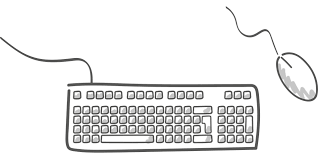
\includegraphics[width=0.3\textwidth]{Figures/mouse1} \quad
	% 
\includegraphics[width=0.2\textwidth]{Figures/toque}
% \end{figure}

\begin{itemize}
	\item Intera��es n�o convencionais:
	\begin{itemize}
		\normalsize
		\smallskip
    \item acionadores externos, \textbf{reconhecimento autom\'atico de voz}, etc.
	\end{itemize}
\end{itemize}
\begin{figure}
	% 
\includegraphics[width=0.2\textwidth]{Figures/talk} \quad
	% 
\includegraphics[width=0.4\textwidth]{Figures/ta} \quad
	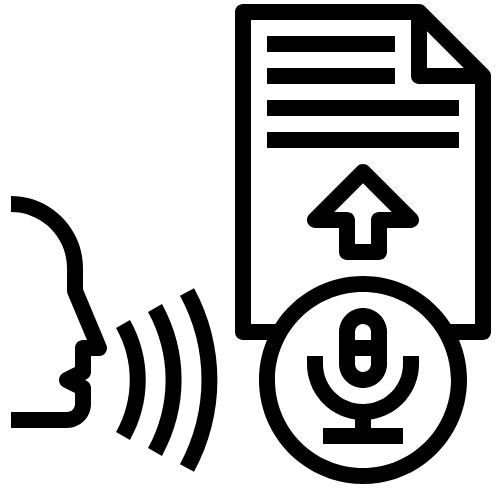
\includegraphics[width=0.2\textwidth]{Figures/icon_asr}
\end{figure}
\end{frame}

% \begin{itemize}
%     \item Aplica��es:
%     \begin{itemize}
%         \item Tecnologias assistivas, \textit{eye-trackers}, estudos em lingu�stica, s�ntese de voz
%     \end{itemize}
% \end{itemize}

% ----------------------------------------------------------------------------
%\begin{frame}{Por que utilizar Acionadores?}
%\begin{itemize}
%	\item Acessibilida
%	\smallskip
%	\item Melhoram a intera��o humano-computador (IHC)
%	\smallskip
%	\item Comodidade e conforto
%\end{itemize}
%\begin{figure}
%	\includegraphics[width=0.48\textwidth]{Figures/jarvis02}
%\end{figure}
%\end{frame}

%%%%%%%%%%%%%%%%%%%%%%%%%%%%%%%%
% \subsection{Motiva��o}
% % ----------------------------------------------------------------------------
% \begin{frame}{Motiva��o}
% \begin{itemize}
% 	\item \textbf{Acessibilidade}: TA para PCD \medskip
% 	\item Tecnologia Assistiva voltada �s pessoas com defici�ncia
% \end{itemize}
% \begin{figure}
% 	
\includegraphics[width=0.80\textwidth]{Figures/access_1}
% \end{figure}
% \end{frame}

% ----------------------------------------------------------------------------
%\begin{frame}{Estat�sticas da Popula��o com Defici�ncia}
%\begin{itemize}
%	\item Mundialmente: 15\% da popula��o $\approx$ 1 bilh�o de
%	pessoas~\textcolor{gray}{\small[OMS, 2015]}
%	\medskip
%	\item No Brasil: 23,9\% dos brasileiros $\approx$ 46 milh�es de
%	pessoas~\textcolor{gray}{\small[IBGE, 2010]}
%\end{itemize}
%\begin{table}
%\centering
%\caption{Perfil da popula��o brasileira com defici�ncia}
%\begin{tabular}{lcr}
%	\hline
%	\hline
%	{\bf Defici�ncia} & {\bf N�mero de Pessoas} & {\bf Porcentagem} \\
%	\hline
%	{Visual}          & {35.774.392}            & {18,754}     \% \\
%	{\bf Motora}      & {\bf 13.265.599}        & {\bf 6,95}   \% \\
%	{Auditiva}        & 9.717.318               & 5,094        \% \\
%	{Cognitiva}       & 2.611.536               & 1,369        \% \\
%	\hline
%	\hline
%\end{tabular}
%\end{table}
%\end{frame}

%\begin{frame}{Problemas}

%    \begin{itemize}
%    \item Intera��es Convencionais for�am o uso das m�os
%    \item Falta de acessibilidade para PCD
%    \item Pre�o dos dispositivos existentes
%    \end{itemize}

%\end{frame}

%\begin{frame}{Dispositivos Dispon�veis - Detector de Pisque}
%	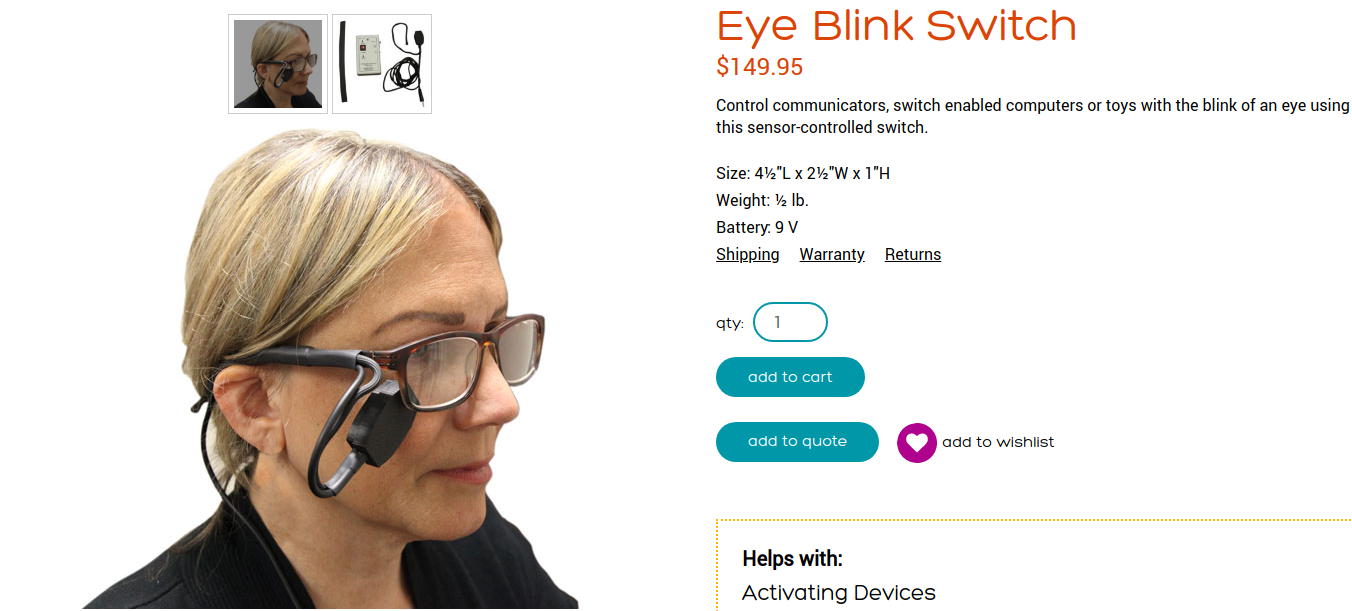
\includegraphics[width=\textwidth]{Figures/blink_switch}
%\end{frame}

%\begin{frame}{Dispositivos Dispon�veis - Detector de Sopro}
%	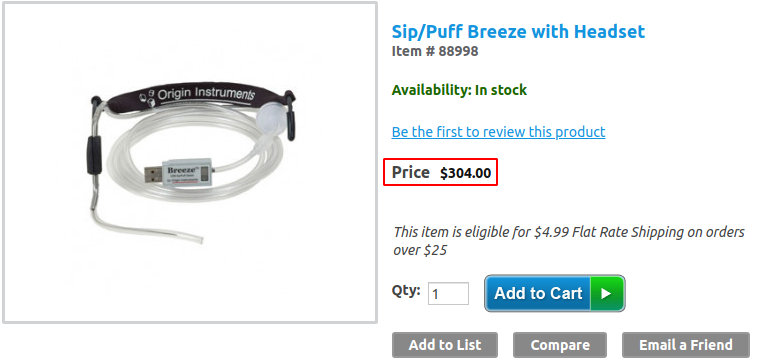
\includegraphics[width=\textwidth]{Figures/puff}
%\end{frame}

%\begin{frame}{Dispositivos Dispon�veis - {Mouse Tracker} com Girosc�pio}
%    \begin{itemize}
%        \item \url{zyteq.com}
%    \end{itemize}
%	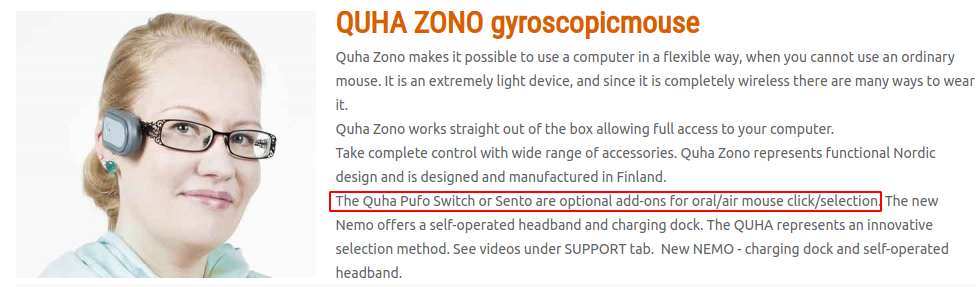
\includegraphics[width=\textwidth]{Figures/zono}
%	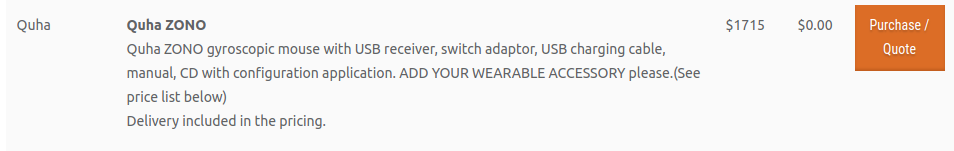
\includegraphics[width=\textwidth]{Figures/price}
%\end{frame}

%\subsection{Proposta}
%% ----------------------------------------------------------------------------
%\begin{frame}{Proposta do Trabalho}
%\begin{itemize}
%	\item Controlador de mouse baseado na cabe�a do usu�rio
%	\begin{itemize}
%		\normalsize
%		\medskip
%		\item[--] M�todo alternativo de clique
%		\item[--] Multiplataforma
%		% \begin{itemize}
%		% 	\normalsize
%		% 	\item[$\hookrightarrow$] Linux
%		% \end{itemize}
%		%\smallskip
%		\item[--] Livre: \textit{open-source} e \textit{open-hardware}
%		\item[--] De baixo custo
%		\smallskip
%		\item[--] Com foco em acessibilidade
%		\begin{itemize}
%			\smallskip
%			\normalsize
%			\item[$\hookrightarrow$] PCD motora dos membros superiores
%			(MMSS)
%            \item[$\hookrightarrow$] Movimento cognitivo e da cabe�a preservado

%		\end{itemize}
%	\end{itemize}
%\end{itemize}
%\end{frame}




%\subsection{Justificativa}
%% ----------------------------------------------------------------------------
%\begin{frame}{Justificativa}
%\begin{itemize}
%\item Por que utilizar o sopro e movimenta��o da cabe�a do usu�rio como m�todo de controle?
%\end{itemize}
%\begin{itemize}
%	\item No meio acad�mico:
%	\smallskip
%	\begin{itemize}
%		\normalsize
%		\item Dificuldade em encontrar trabalhos que utilizam
%acionadores como m�todo alternativo de clique e movimenta��o do mouse
%		\smallskip
%		\item Apenas um trabalho de acionador externo baseado em
%sopro~\textcolor{gray}{\small[B. Aigner, 2016]}
%		\smallskip
%		\item  Poucos detalhes do desenvolvimento de
%		acionadores externos
%		\smallskip
%	\end{itemize}
%\end{itemize}

%\end{frame}


%\begin{frame}{Justificativa}
%%
%\begin{itemize}
%	\item No mercado:
%	\smallskip
%%\begin{minipage}{0.65\textwidth}
%\begin{itemize}
%	\item[]
%\begin{itemize}
%	\normalsize
%	\item  Comunica��o direta atrav�s da interface de �udio para realizar o clique
%	\smallskip
%	\item  Acionadores externos de alto custo e propriet�rios
%\end{itemize}
%\end{itemize}
%\end{itemize}
%%\end{minipage}
%\begin{figure}
%	\centering
%	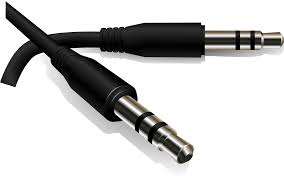
\includegraphics[width=0.3\textwidth]{Figures/ts1}\\
%	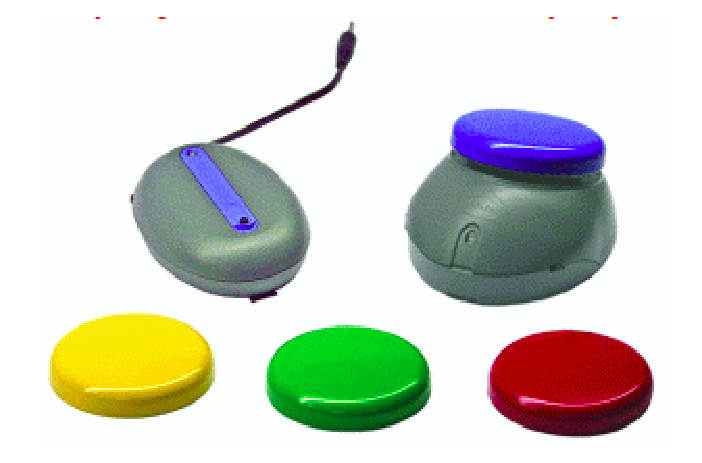
\includegraphics[width=0.3\textwidth]{Figures/at_switch_wireless} \quad
%	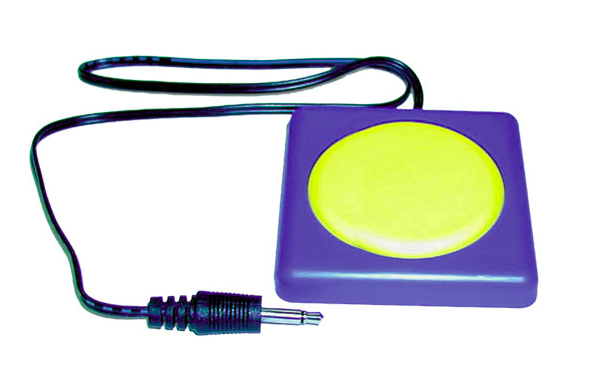
\includegraphics[width=0.3\textwidth]{Figures/at1}
%\end{figure}
%\end{frame}
%%% EOF %%%


\section{Prot�tipo}
%%%%%%%%%%%%%%%%%%%%%%%%%%%%%%%%
\subsection{Objetivos}
% ----------------------------------------------------------------------------
\begin{frame}{Reconhecimento de Voz}

\begin{figure}
	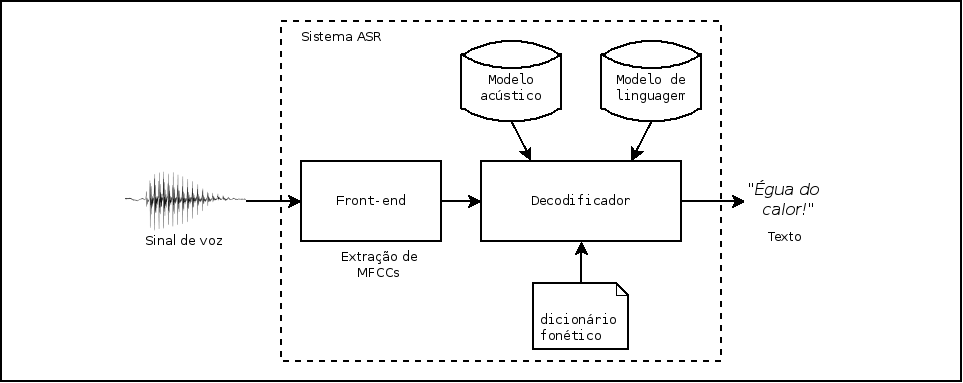
\includegraphics[width=0.9\textwidth]{Figures/asr}
    \caption{Esquema tradicional de um sistema autom\'atico de reconhecimento de voz}
\end{figure}

\begin{itemize}
    \item Aplica\c c\~oes:
    \begin{itemize}
        \smallskip
		\item Tecnologias assistivas, \textit{eye-trackers}, lingu\'istica (\textbf{alinhamento fon\'etico}), s\'intese de voz
    \end{itemize}
\end{itemize}
\end{frame}


\begin{frame}
\frametitle{Alinhamento Fon\'etico For\c cado}
	\begin{itemize}
		\item Automatiza\c c\~ao  da transcri\c c\~ao e alinhamento de fala gravada
		\item Estudo e pesquisa de fon\'eticos
		\item Desenvolvimento de ferramentas mais robustas de reconhecimento e sintese de fala
	\end{itemize}
	\begin{figure}
	\begin{center}
		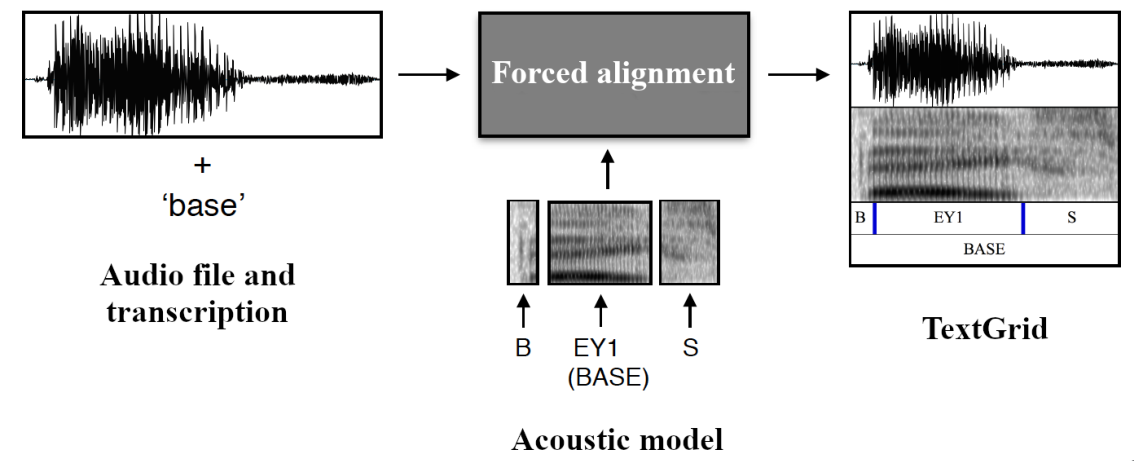
\includegraphics[width=0.8\textwidth]{Figures/align}
	\end{center}
	\end{figure}


\end{frame}


\begin{frame}{Ferramentas}
    \begin{itemize}
        \item Kaldi: um pacote \textit{open-source} de reconhecimento de voz
			\begin{itemize}
				\item Possui suporte para ambas HMM-GMMs (mistura de gaussianas) e HMM-DNNS (redes neurais profundas)
				\item Suporte para PT-BR
			\end{itemize}
		\begin{figure}
		\begin{center}
			
\includegraphics[width=0.4\textwidth]{Figures/kaldi}
		\end{center}
		\end{figure}

        \item Praat: \textit{software} utilizado por linguistas na  an\'alise da fala

    \end{itemize}
\end{frame}


\begin{frame}{Objetivo}
\begin{itemize}
    % \item Desenvolver um sistema de reconhecimento de voz para PT\_BR utilizando o pacote Kaldi para treinamento dos AMs e LMs
	\item Desenvolver um alinhador fon\'etico para PT\_BR utilizando o pacote de ferramentas Kaldi
	\begin{itemize}
		\item \textit{Plug-in} para o Praat
		\item Modelos ac\'usticos (AMs) treinados utilizando DNNs e HMM-GMMs
	\end{itemize}
	\item Coletar dados para realizar \textit{LM rescoring}: 4-5 milh\~oes de frases
    \item Disponibilizar recursos \`a comunidade cient\'ifica: grupo Fala Brasil
\end{itemize}

\begin{figure}
\begin{center}
	
\includegraphics[width=0.3\textwidth]{Figures/falabrasil}
\end{center}
\end{figure}

\end{frame}

%
\section{Testes e Resultados}
%% ----------------------------------------------------------------------------
%\begin{frame}{Agenda}
%\begin{enumerate}
%	\setcounter{enumi}{3}
%	\item Ambiente de Teste e Resultados Preliminares
%	\bigskip
%	\begin{itemize}
%		\item Avalia��es: objetiva e subjetiva
%		\bigskip
%		\item Perfil dos volunt�rios 
%		\bigskip
%		\item Resultados preliminares com o AGR
%	\end{itemize}
%\end{enumerate}
%\end{frame}

%%%%%%%%%%%%%%%%%%%%%%%%%%%%%%%%
\subsection{Testes}
\begin{frame}{Participantes}

\begin{itemize}
    \item 20 participantes: Estudantes de gradua��o ou p�s-gradua��o da UFPA
    % \item Exig�ncia m�nima: familiaridade com os \textit{websites} escolhidos no teste 
    \item Termo de consentimento
\end{itemize}

\end{frame}

\begin{frame}{Dwell Time e eViacam}
    \begin{figure}
        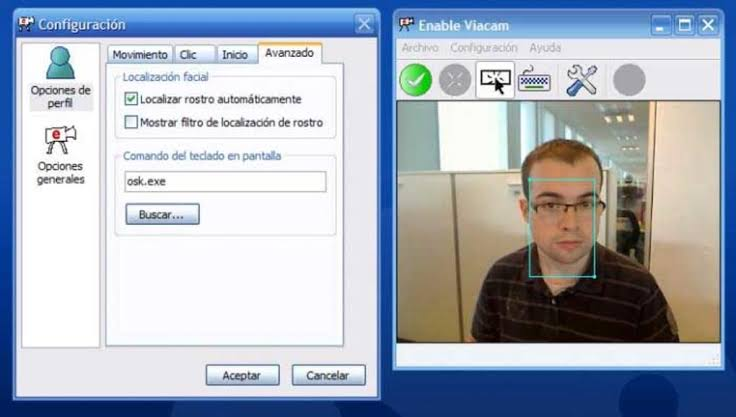
\includegraphics[width=0.9\linewidth]{Figures/eviacam}
    \end{figure}
\end{frame}

\begin{frame}{Ambiente de Teste}
\begin{itemize}
\item Ambiente bem iluminado
\item Cadeira de frente para um \textit{laptop} equipado com {webcam}
% \item Dois m�todos de clique: Baseado em sopro e \textit{dwell time}
\item (\textit{Dwell time + Eviacam}) X (Sopro + Giroscopio/Aceler�metro)
\end{itemize}
\end{frame}


\begin{frame}{Tarefas}
    \begin{itemize}
        \item Testes realizados no \textit{website} G1
        \item[--] Dificuldade na utiliza��o para PCD
    \end{itemize}
	\begin{figure}
		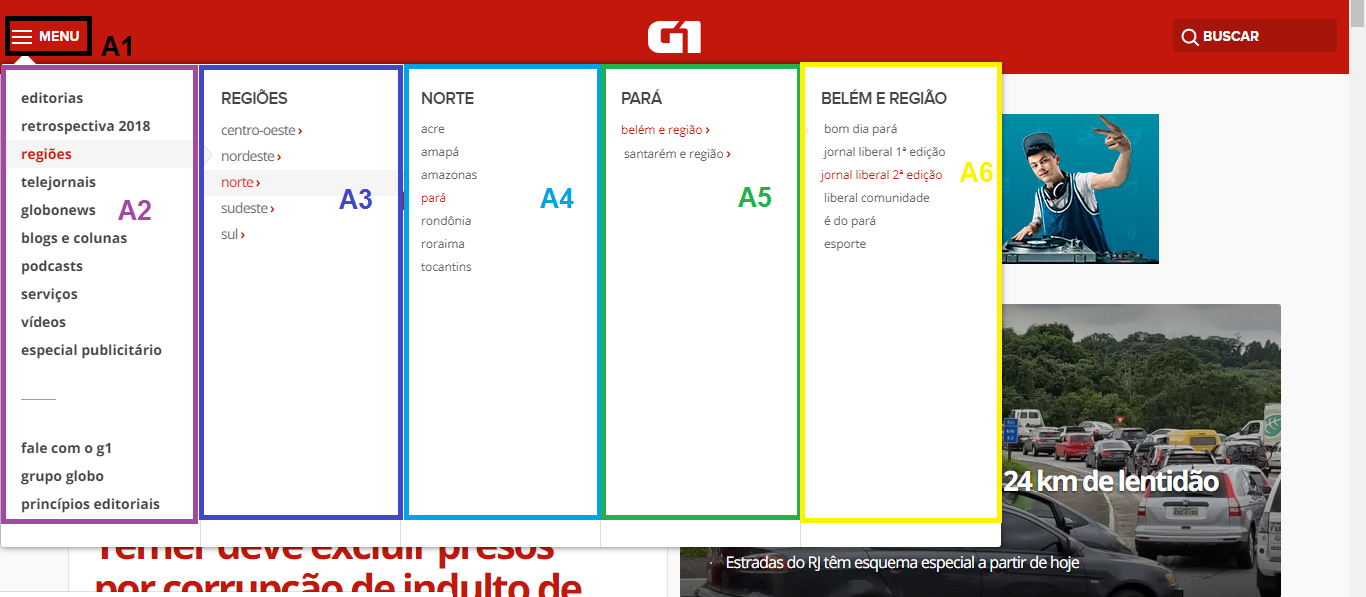
\includegraphics[width=\linewidth]{Figures/g1_areas}
        \caption{�reas de interesse destacadas pelos ret�ngulos A1, A2, etc.}
	\end{figure}

\end{frame}



\begin{frame}{Avalia��es}
\begin{itemize}
\item \textbf{Quantitativa}: Tempo de execu��o e erros de cliques   
\item \textbf{Qualitativa}: Question�rio objetivo com 6 quest�es
\item \textbf{Subjetiva}: Pergunta subjetiva sobre o dispositivo de sopro 
\end{itemize}

\end{frame}





\subsection{Resultados Quantitativos}
\begin{frame}{Resultados Quantitativos [1/2]}
	\centering
	\begin{figure}
		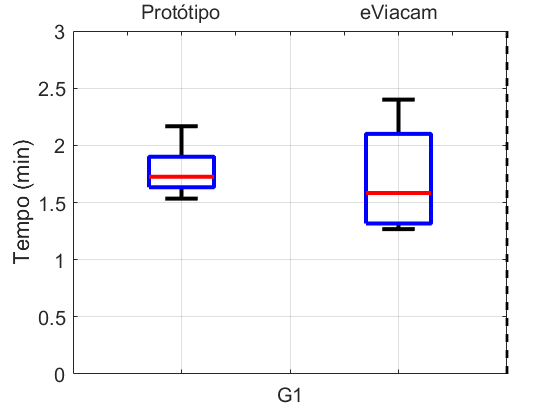
\includegraphics[width=0.8\textwidth]{Figures/tempo_g1}
		\caption{Tempo de execu��o das tarefa.}
	\end{figure}
\end{frame}

\begin{frame}{Resultados Quantitativos [2/2]}
	\centering
	\begin{figure}
		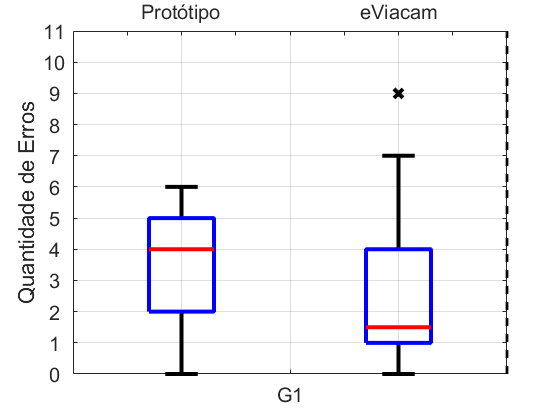
\includegraphics[width=0.8\textwidth]{Figures/erros_g1}
		\caption{Erros de cliques cometidos.}
	\end{figure}
\end{frame}

% \begin{frame}{Resultados Quantitativos [3/3]}
% 	\begin{figure}
	
% 	\makebox[\linewidth]{\parbox{12cm}{  %{\lipsum}}
% 		\subfloat[Dwell time.]{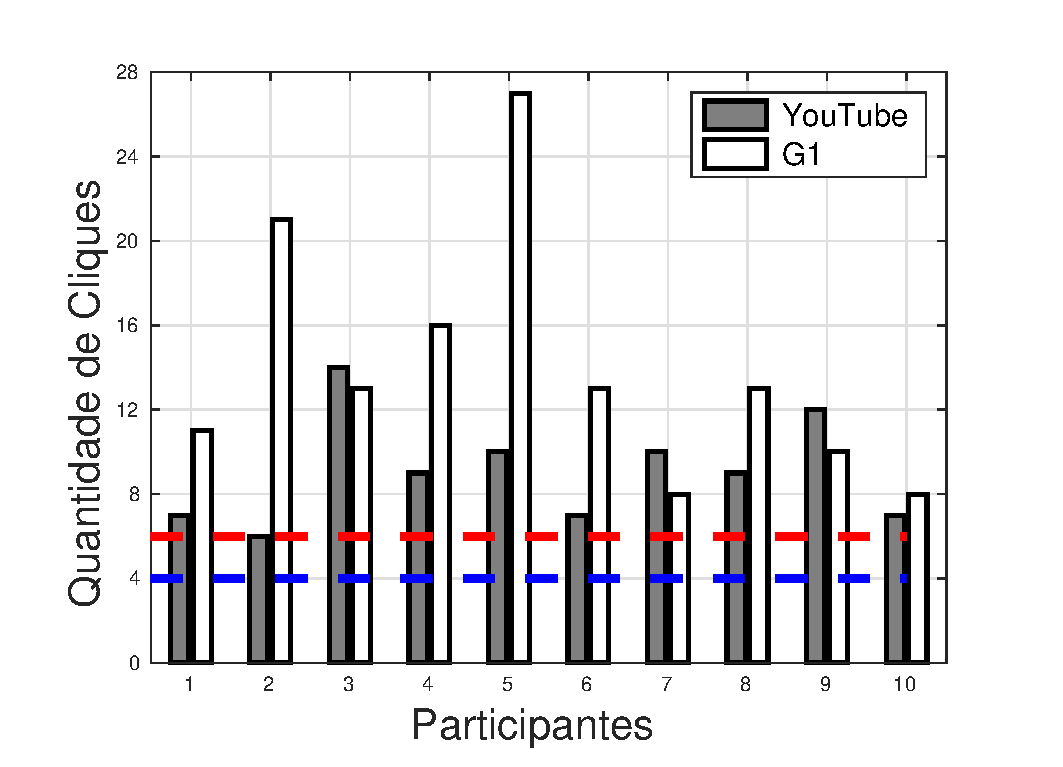
\includegraphics[width=0.5\linewidth]{Figures/DwellClicks}} \quad
% 		\subfloat[Sopro.]{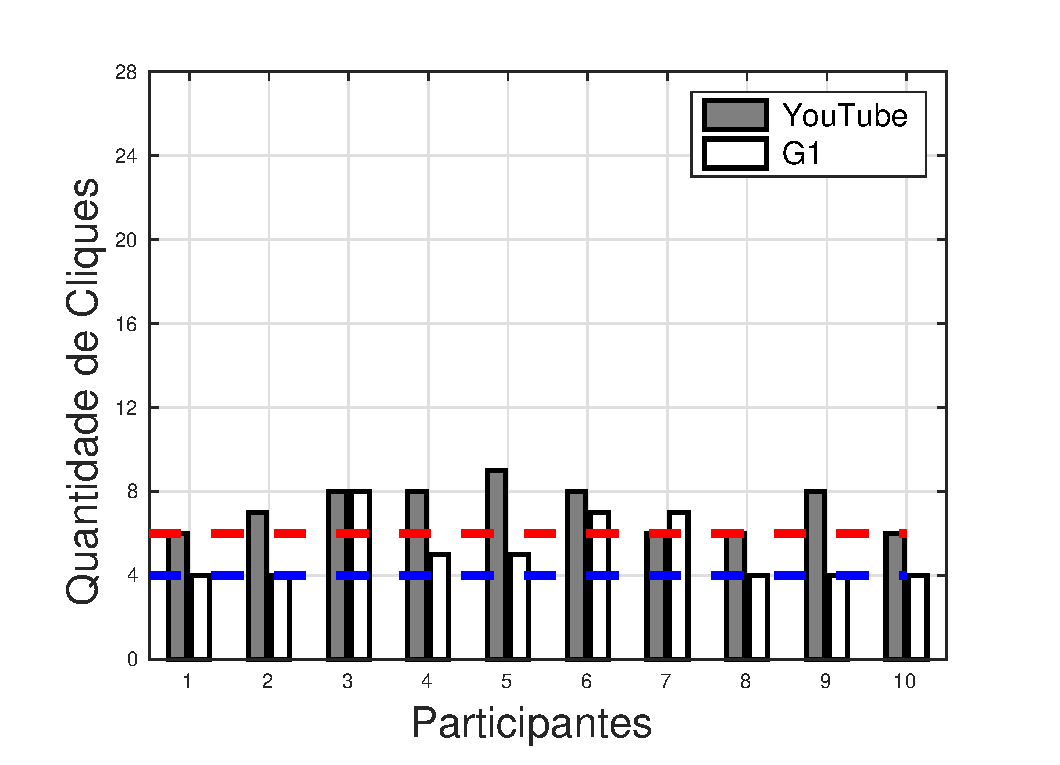
\includegraphics[width=0.5\linewidth]{Figures/PuffClicks}}
% }}
% 	\end{figure}

% \end{frame}

\subsection{Resultados Qualitativos}
\begin{frame}{Question�rio Objetivo}
\begin{table}[!t]
\centering
\begin{tabular}{cc|ll}
	\hline
	\hline
	~ & \textbf{Pergunta} & \multicolumn{2}{c}{\textbf{Resposta}} \\
	\hline \textbf{1} & Experi�ncia de uso & 1 -- insuficiente & 5 -- excelente \\
	\textbf{2} & Tempo & 1 -- lento & 5 --  r�pido \\
	\textbf{3} & Precis�o& 1 -- insuficiente & 5 -- excelente \\
	\textbf{4} & Esfor�o cognitivo& 1 -- alto & 5 -- baixo\\
	\textbf{5} & Esfor�o f�sico & 1 -- alto & 5 --  baixo\\
	\textbf{6} & Concentra��o & 1 -- mais no clique & 5 -- mais na tarefa \\
	\hline
	\hline
\end{tabular}
\end{table}

\begin{minipage}{.1\textwidth} 

\end{minipage}
\noindent\hspace{0.28\linewidth}\begin{minipage}{.7\textwidth} 
\begin{itemize}
\item[\textcolor{black}{$\blacksquare$}]   Escala Likert
\begin{itemize}
\item[\textcolor{red}{$\blacksquare$}] 1 --- Muito Ruim 
\item[\textcolor{orange}{$\blacksquare$}] 2 --- Ruim       
\item[\textcolor{yellow}{$\blacksquare$}]   3 --- Regular    
\item[\textcolor{erick}{$\blacksquare$}]   4 --- Bom        
\item[\textcolor{suzane}{$\blacksquare$}] 5 --- Muito Bom  
\end{itemize}
\end{itemize}
\end{minipage}
\begin{minipage}{.1\textwidth}

\end{minipage}

\end{frame}


\begin{frame}{Question�rio Objetivo - An�lise}
	
	% \begin{figure}
	% 	\begin{minipage}{.85\textwidth}
	% 	\subfloat{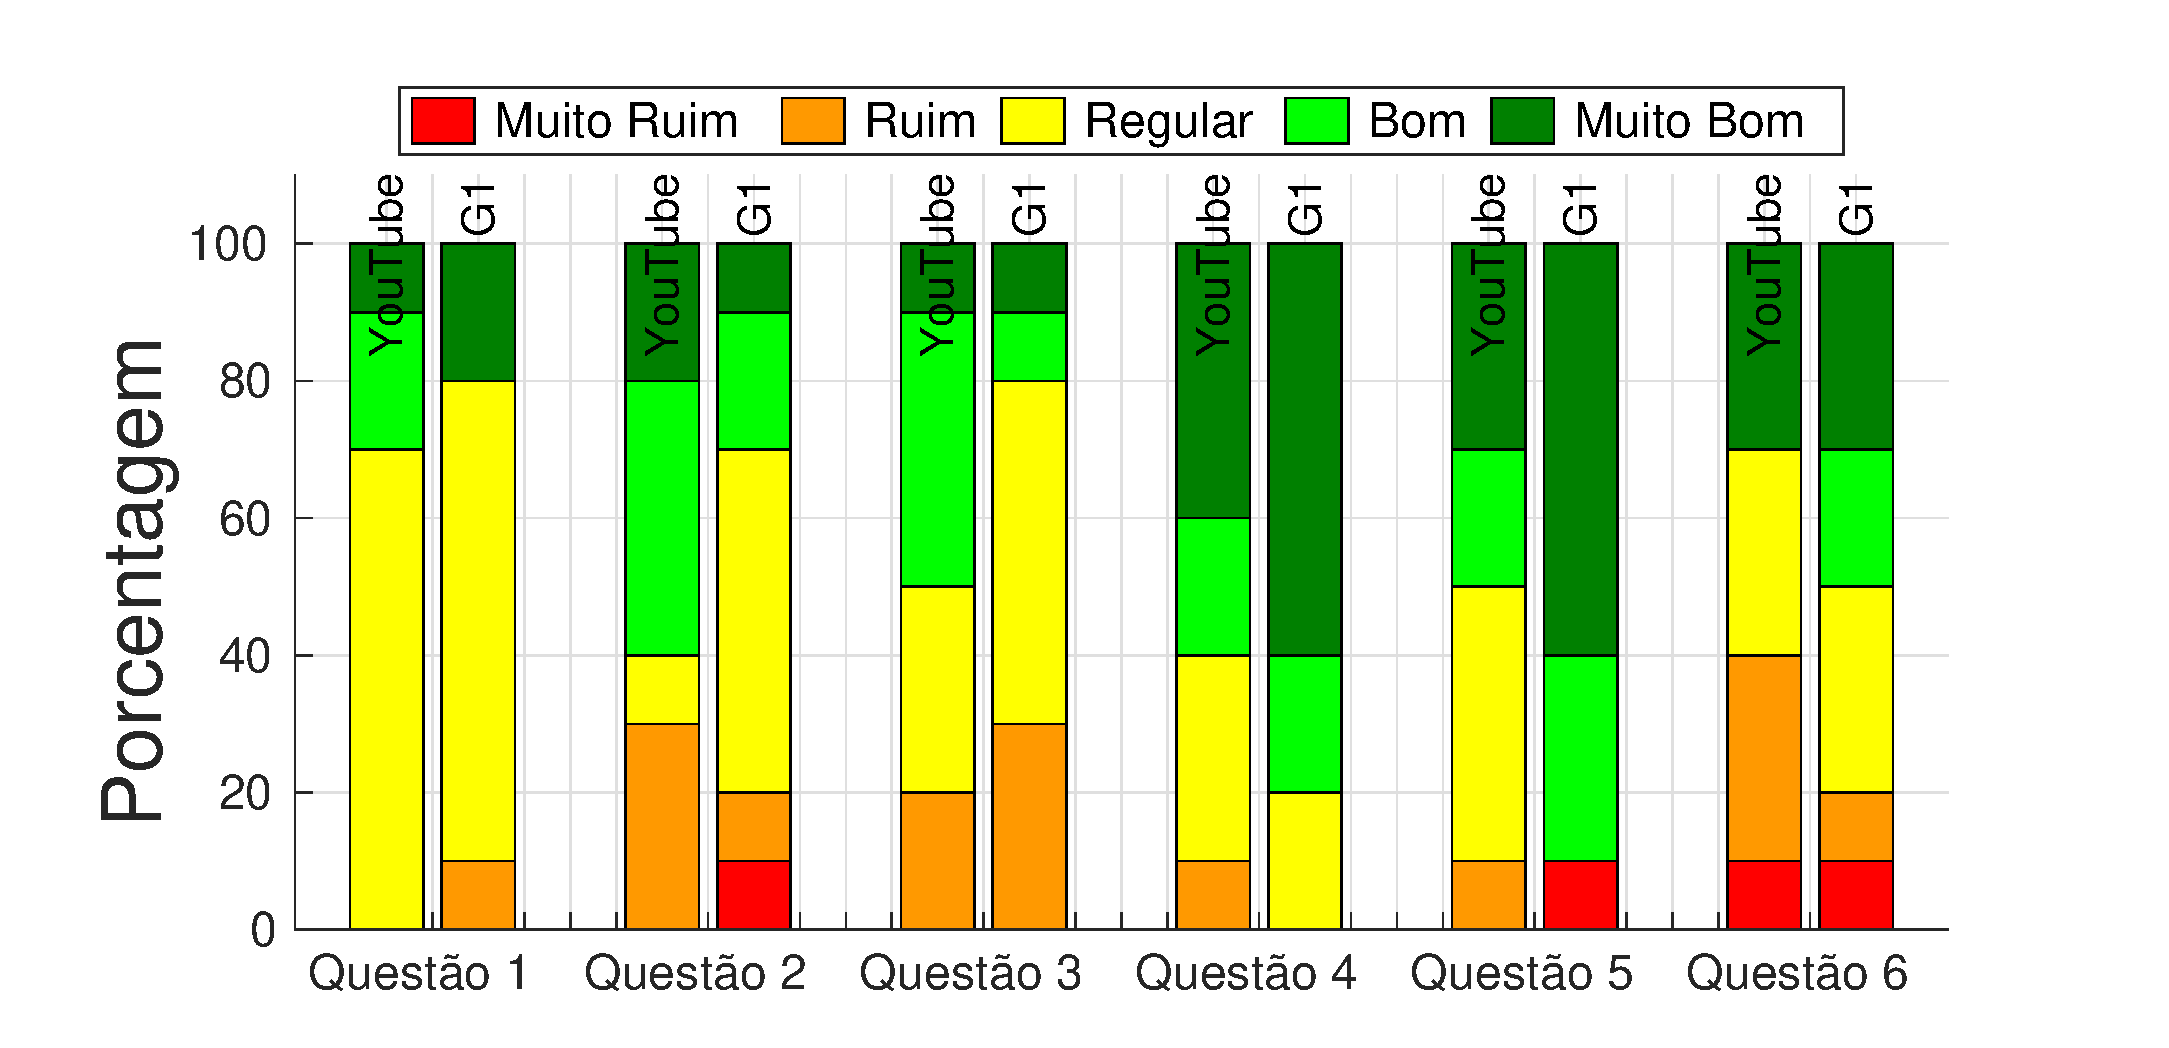
\includegraphics[width=0.95\linewidth]{Figures/DwellQuestions}}\\
	% 	\end{minipage}
	% 	\begin{minipage}{.1\textwidth}
	% 	\textit{Dwell time}
	% 	\end{minipage}

	% 	\begin{minipage}{.85\textwidth}
	% 	\subfloat{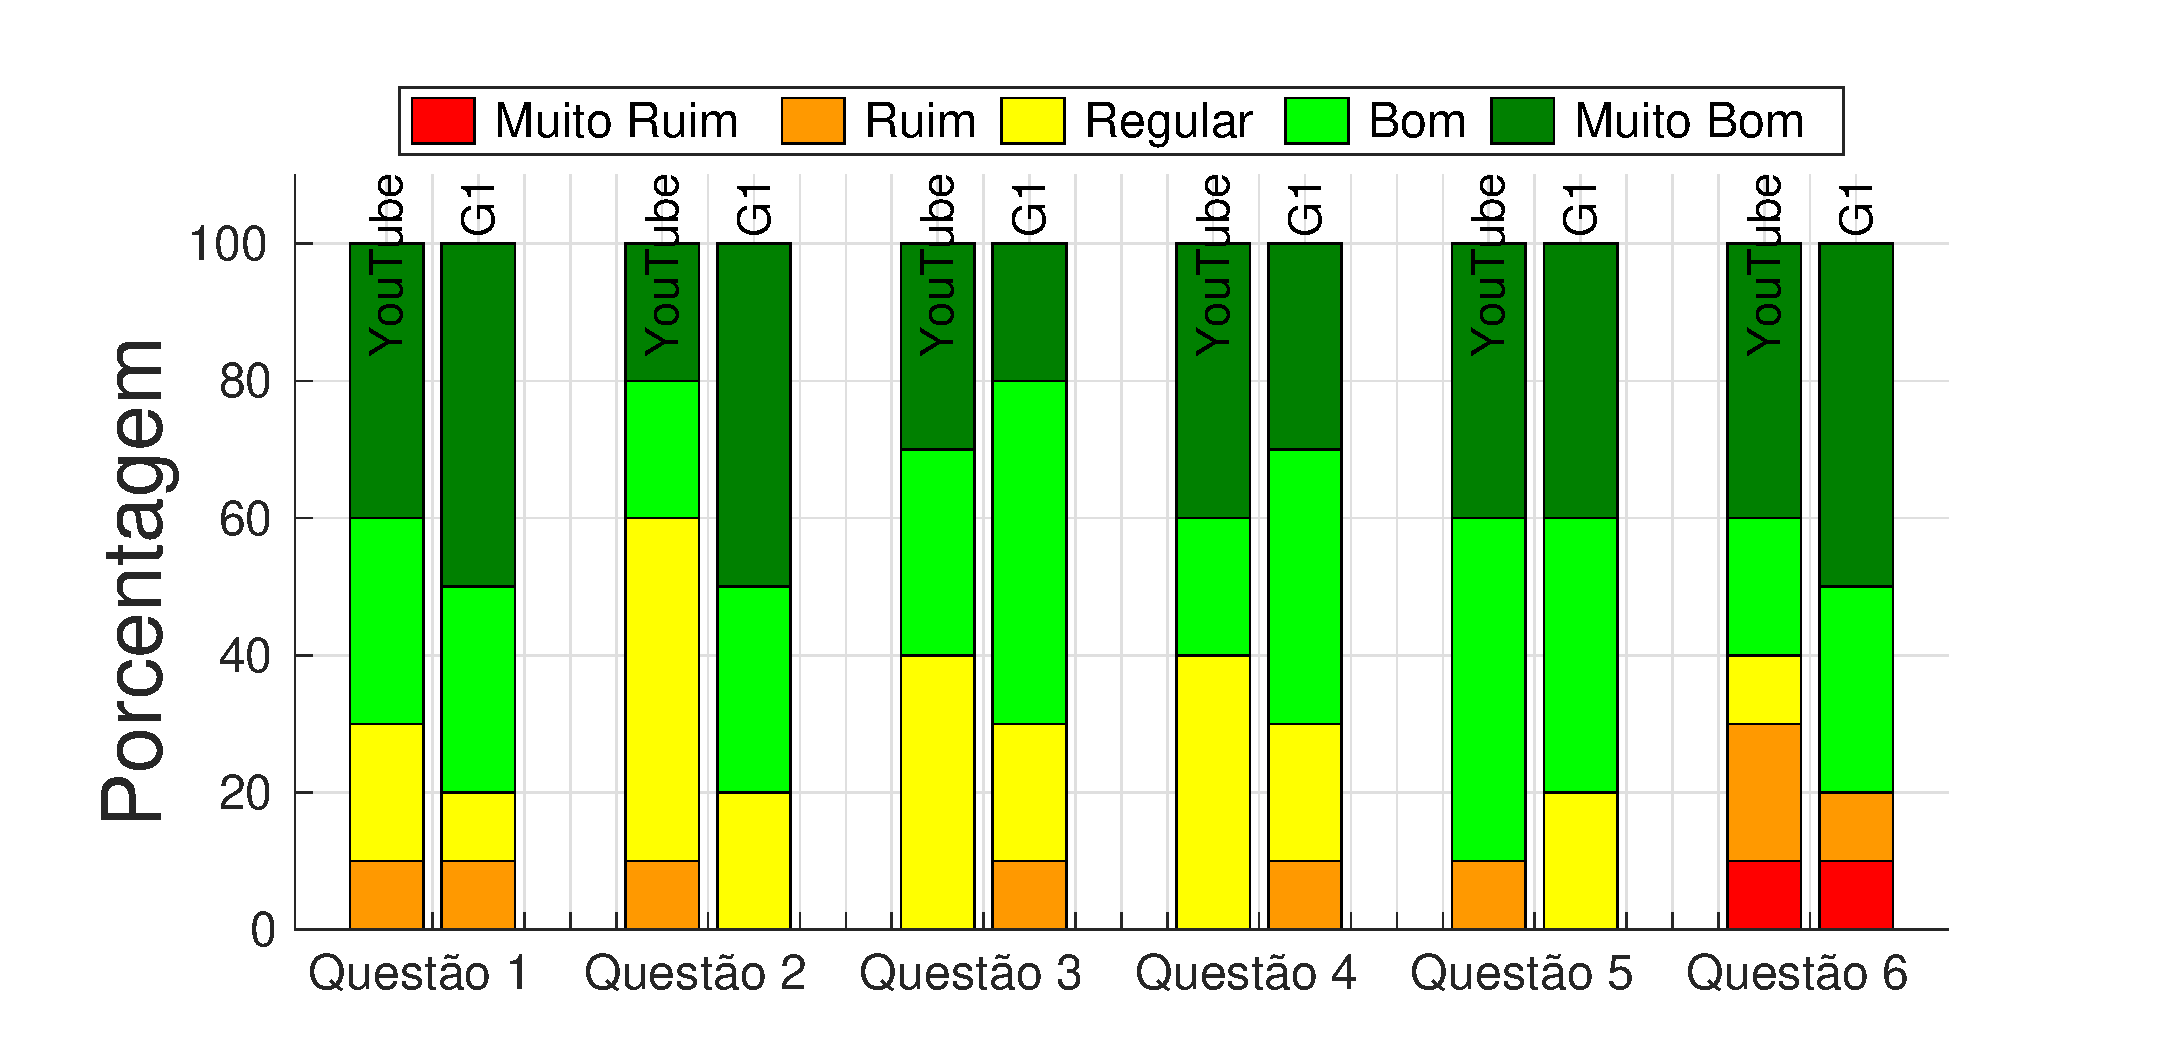
\includegraphics[width=0.95\linewidth]{Figures/PuffQuestions}}
	% 	\end{minipage}
	% 	\begin{minipage}{.1\textwidth}
	% 	Sopro
	% 	\end{minipage}
	% \end{figure}

    \begin{figure}
        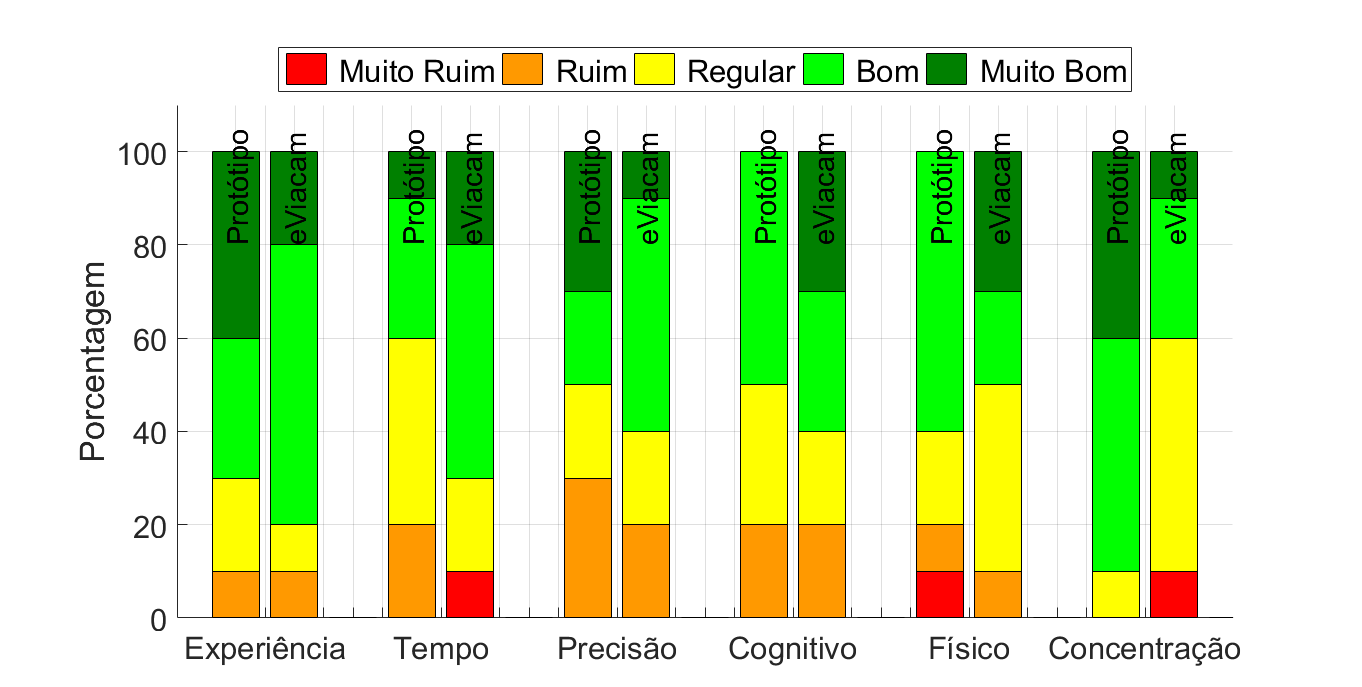
\includegraphics[width=\linewidth]{Figures/likert}
        \caption{Escala Likert para prot�tipo e eViacam}
    \end{figure}

\end{frame}

% \begin{frame}{An�lise dos Resultados}
%     \begin{itemize}
        % \item 
% \end{frame}

\subsection{Quest�o Subjetiva}
\begin{frame}{Discuss�o Sobre a Quest�o Subjetiva}

\begin{center}
\textbf{``Com base na sua experi�ncia de uso, que sugest�es voc� daria para melhoria do dispositivo?''}
\end{center}

\begin{itemize}
\item Cliques involunt�rios
\item Centraliza��o do cursor
\item Substitui��o do \textit{headset}
\item Sensibilidade ajust�vel
\item \textit{Feedback} visual a fim de mostrar o n�vel de sensibilidade
\end{itemize}

\end{frame}

%
\section{Considera��es Finais}
%% ----------------------------------------------------------------------------
%\begin{frame}{Agenda}
%\begin{enumerate}
%	\setcounter{enumi}{4}
%	\item Considera��es
%	\bigskip
%	\begin{itemize}
%		\item Discuss�o dos resultados preliminares
%		\bigskip
%		\item Trabalhos futuros
%		\bigskip
%		\item Contribui��es e conquistas
%	\end{itemize}
%\end{enumerate}
%\end{frame}

%%%%%%%%%%%%%%%%%%%%%%%%%%%%%%%%
\subsection{Considera��es Finais}
% ----------------------------------------------------------------------------
\begin{frame}{Considera��es Finais}
\begin{itemize}
\item Proposta \textit{open-source} de baixo custo: \url{https://github.com/bg34r/HeadMousino}
\item Dispositivo de prop�sito geral
\item Uma boa alternativa ao \textit{dwell time} e ao eViacam
    \begin{itemize}
        \normalsize
        % \smallskip
        \item[--] Usu�rios com �culos
        \item[--] Ambientes pouco iluminados
        \item[--] Necessidade de uma \textit{webcam}
        \item[--] Sigaa, YouTube, etc.
    \end{itemize}
% \item Dispon�vel abertamente em: \url{https://github.com/ErickCampos/At-Switch}
\end{itemize}
\end{frame}

%%%%%%%%%%%%%%%%%%%%%%%%%%%%%%%%

% \subsection{Contribui��o}
% \begin{frame}{Contribui��o}

% \begin{figure}
% 	\centering
% 	
\includegraphics[width=0.3\linewidth]{Figures/ihclogo.png}
% \end{figure}

% \begin{itemize}
% \item IHC 2018 - XVII Simp�sio Brasileiro sobre Fatores Humanos em Sistemas
% Computacionais
% \bigskip
% \item \textit{``A Non-Conventional Interaction on Computational Systems Based on Mouth Puffing''}
% \end{itemize}

% \end{frame}


\subsection{Trabalhos Futuros}
% ----------------------------------------------------------------------------
\begin{frame}{Trabalhos Futuros}
\begin{itemize}
% \item Expandir para outros sistemas operacionais: Windows, MacOS Android
\item Solu��o alternativa ao \textit{headset}
\item Sensores alternativos: Microfones de eletreto, BMP180 (press�o)
\end{itemize}
\end{frame}
%%% EOF %%%


%%%%%%%%%%%%%%%%%%%%%%%%%%%%%%%%%%%%%%%%%
%%% end of body
%%%%%%%%%%%%%%%%%%%%%%%%%%%%%%%%%%%%%%%%%

\section*{}
\renewcommand*{\currentname}{Agradecimentos}
% ------------------------------------------------------------------------------
\begin{frame}{Agradecimentos}
\begin{figure}
	\centering
	
\includegraphics[width=0.3\textwidth]{Figures/logo_ufpa}
	% 
\includegraphics[width=0.4\textwidth]{Figures/propesp} \quad 
	% 
\includegraphics[width=0.4\textwidth]{Figures/pibic} 
	
\includegraphics[width=0.4\textwidth]{Figures/pibex2} 
\end{figure}



%\begin{center}
%\begin{figure}
%	
\includegraphics[width=0.20\textwidth]{Figures/calabriano}
%	\quad\quad
%	
\includegraphics[width=0.25\textwidth]{Figures/appd}\\[12pt]
%	
\includegraphics[width=0.20\textwidth]{Figures/logo_ufpa}
%	\quad\quad
%	
\includegraphics[width=0.30\textwidth]{Figures/cnpq}
%\end{figure}
%\end{center}
\end{frame}
% ------------------------------------------------------------------------------

% ------------------------------------------------------------------------------
%\begin{frame}{Agradecimentos}
%\begin{center}
%\begin{figure}
%	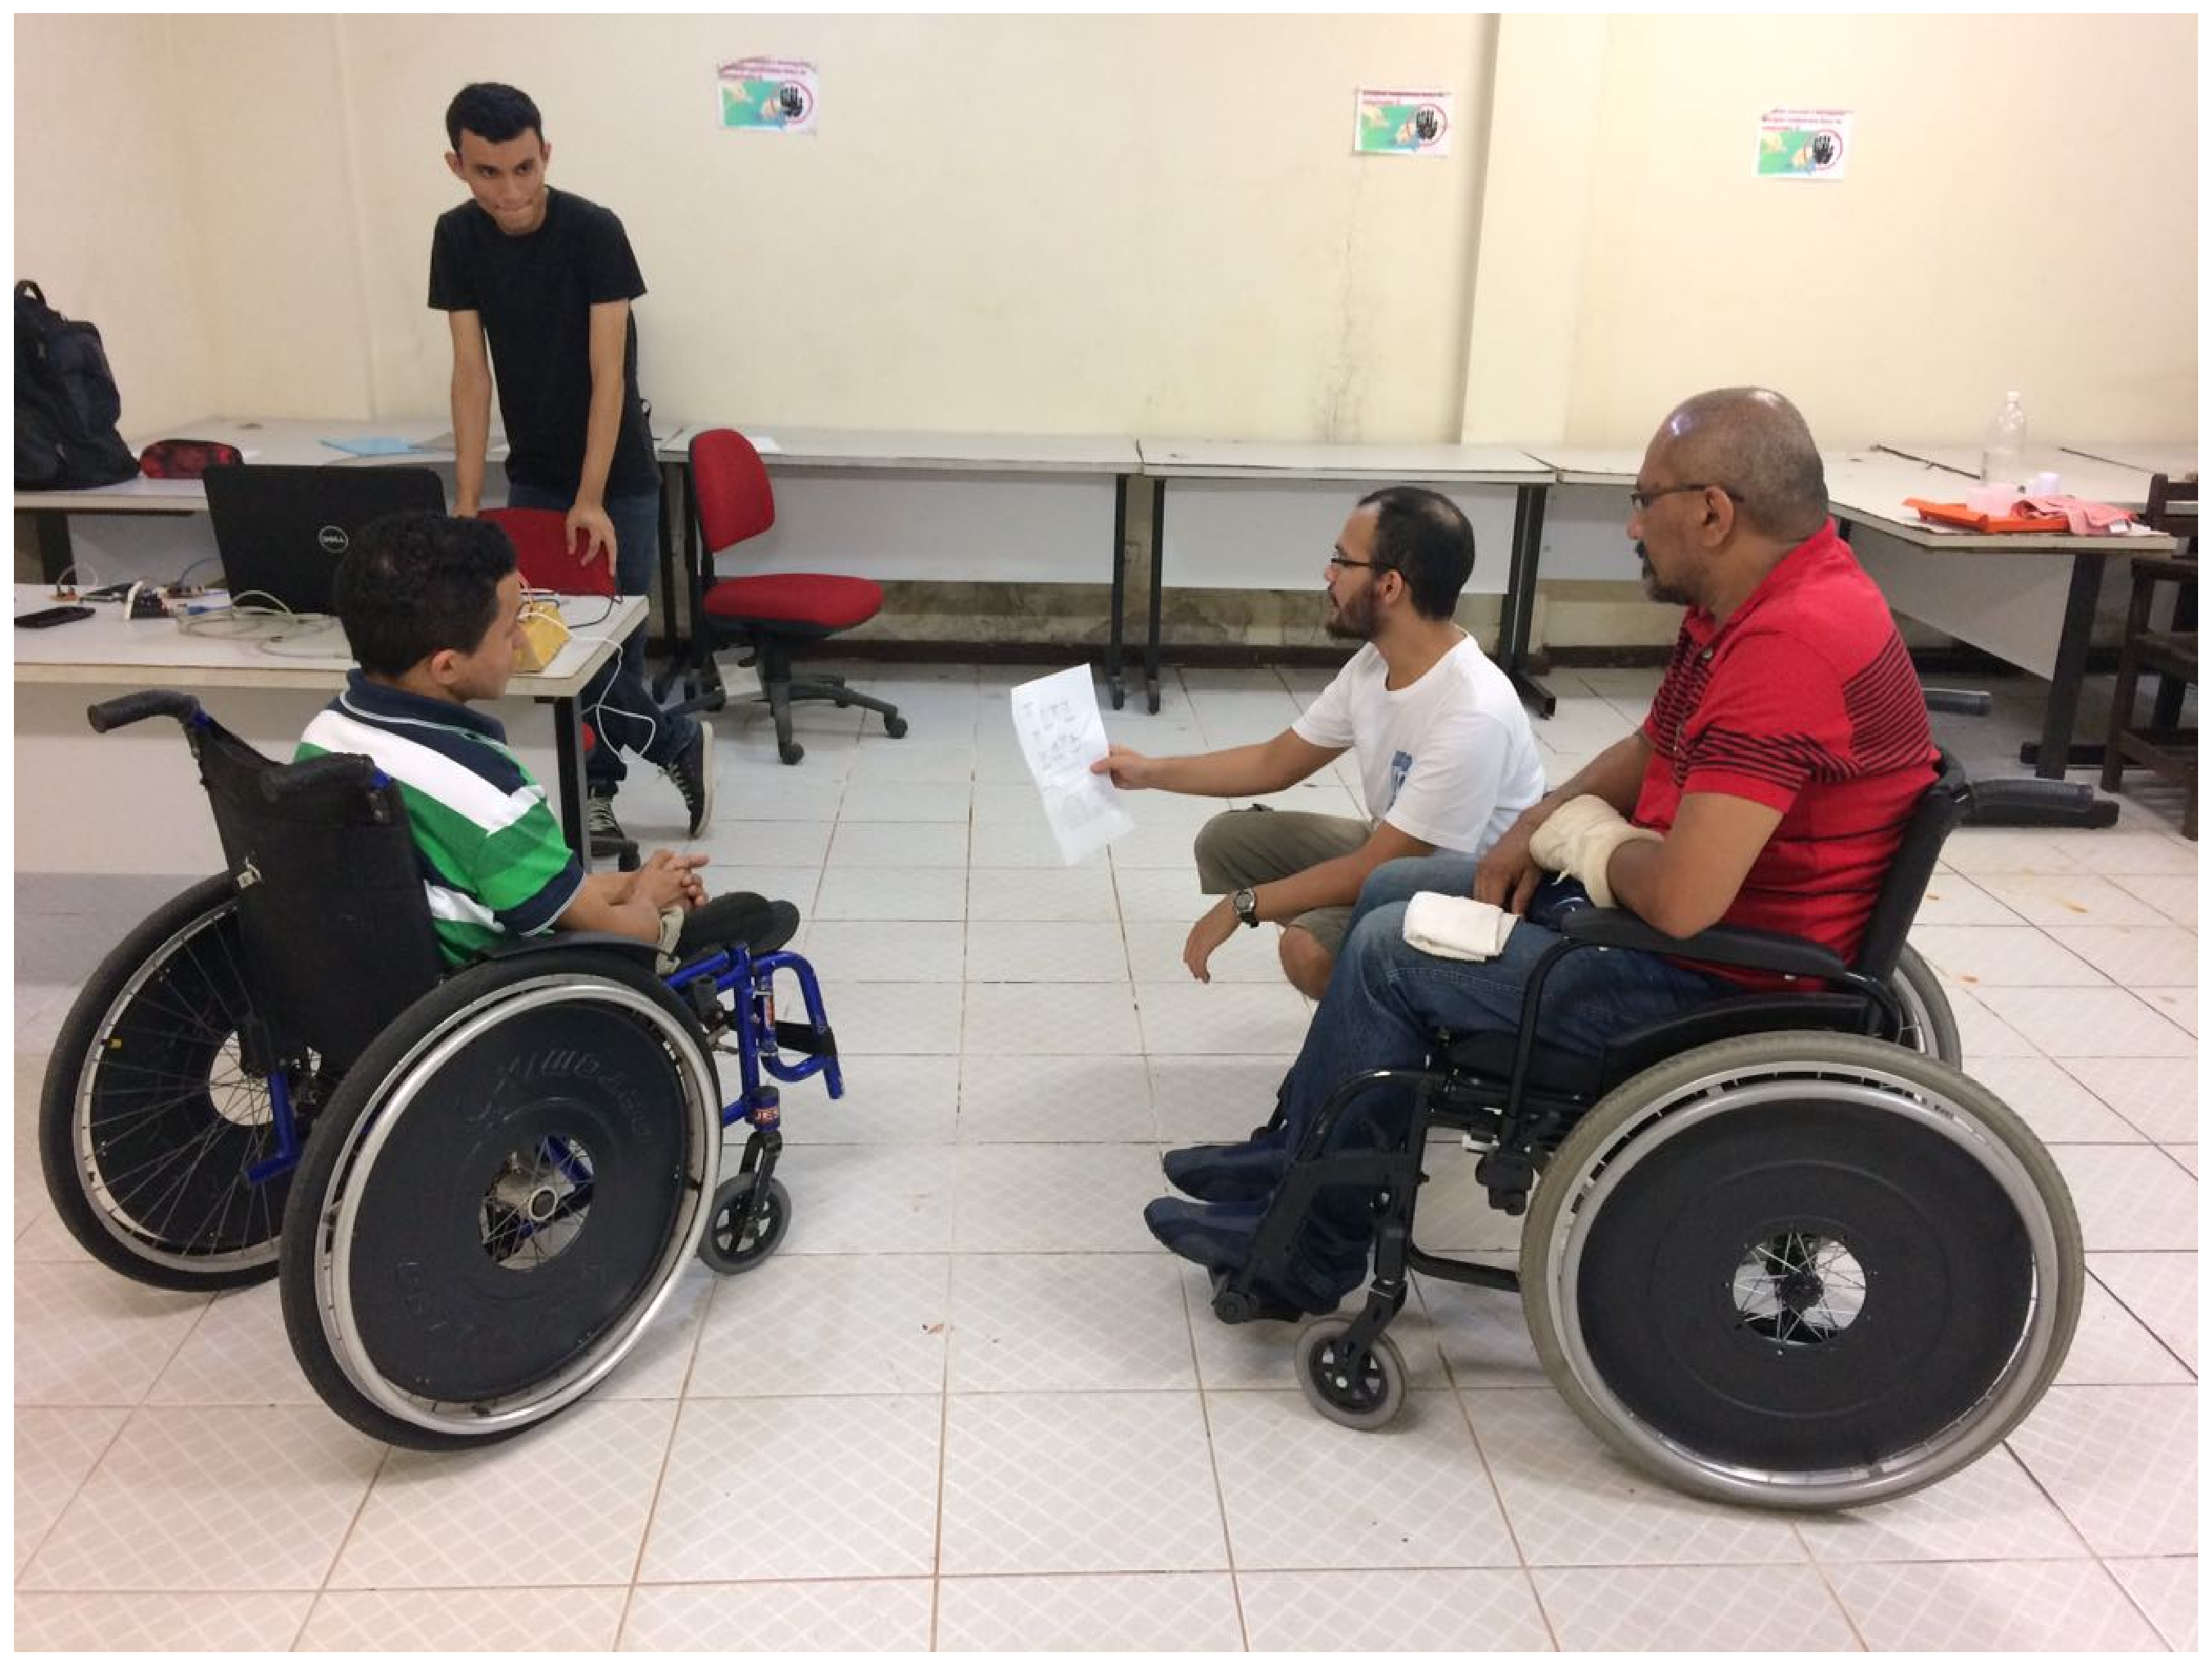
\includegraphics[width=0.85\textwidth]{Figures/voluntarios}
%\end{figure}
%\end{center}
%\end{frame}
% ------------------------------------------------------------------------------

\section*{}
\renewcommand*{\currentname}{Thanks}
%\setbeamertemplate{footline}
%{%
%	\begin{beamercolorbox}[wd=\paperwidth,ht=0.5ex,dp=0ex,center]{footlinerule}
%	\end{beamercolorbox}%
%	\begin{beamercolorbox}[wd=\paperwidth,ht=0.6ex,dp=0ex,center]{empty}
%	\end{beamercolorbox}%
%	\leavevmode%
%	\hbox{%
%
%	\begin{beamercolorbox}[wd=.20\paperwidth,ht=2.25ex,dp=2ex,center]{author in head/foot}%
%		\usebeamerfont{author in head/foot}%
%		%\insertshortauthor\hspace{1em}
%	\end{beamercolorbox}%
%
%	\begin{beamercolorbox}[wd=.45\paperwidth,ht=2.25ex,dp=2ex,right]{title in head/foot}%
%		\usebeamerfont{title in head/foot}
%		%\insertshorttitle
%	\end{beamercolorbox}%
%
%	\begin{beamercolorbox}[wd=.20\paperwidth,ht=2.25ex,dp=2ex,right]{author in head/foot}%
%		\usebeamerfont{author in head/foot}%
%		\textbf{\textcolor{black}{\currentname}}
%	\end{beamercolorbox}%
%
%	\begin{beamercolorbox}[wd=.10\paperwidth,ht=2.25ex,dp=2ex,right]{date in head/foot}%
%		\textbf{\textcolor{black}{\insertframenumber{} of \inserttotalframenumber\hspace*{1ex}}}
%	\end{beamercolorbox}}%
%	\vskip0pt%
%}%
% ------------------------------------------------------------------------------
\begin{frame}
\author{}
\institute{
	\fontsize{34pt}{34pt}\selectfont
	\textcolor{blue!50!black}{\bf Obrigado!}\\[12pt]
}
\date{
	\normalsize
	Jo�o Canavarro (\href{mailto:jvcanavarro@ufpa.br}{\tt jvcanavarro@ufpa.br})\\[1pt]
	Universidade Federal do Par� (UFPA)\\[1pt]
	Bel�m -- Par� -- Brasil\\
}
\titlepage
\end{frame}
\end{document}
%%% EOF %%%
